% Document template
\documentclass[a4paper,11pt, hidelinks]{article}

% Image packages
\usepackage{graphicx, pgf, tikz, pgfplots} 

\usepackage{fancyhdr}						% import fancy hdr
\usepackage{msdata}							% import mathscapes data
\usepackage{hyperref}
\usepackage{background}

\SetBgContents{ }

% Set contents
\SetBgColor{red}
\SetBgPosition{current page.west}% Select location
\SetBgVshift{-1.8cm}
\SetBgOpacity{1}% Select opacity
\SetBgAngle{90.0}% Select rotation of logo
\SetBgScale{1.2}% Select scale factor of logo
\SetBgAnchor{}

% Set date
\usepackage{datetime}						% import datetime package
\newdate{date}{21}{06}{2018}				% set new date
\date{\displaydate{date}}					% configure doc date to new date

% Meta parameters
\setlength{\parindent}{0em}					% remove paragraph indent
\setlength{\parskip}{0.5em}					% set spacing after paragraph
\graphicspath{ {images/} }					% set images path
\fancyhf{}									% clear all header and footers
\renewcommand{\headrulewidth}{0pt}			% remove the header rule
\rfoot{\thepage}					% set page number in right footer


% Copyright message
\chead{}
\lfoot{\mscpy}
\AtEndDocument{\lfoot{}}
\pagestyle{fancy}							% set page styles as fancy

% Document Title
\title{A Micromechanic-based approach towards the Response of Fiber-reinforced Composite Laminates under ballistic impact and blast loading}
\author{ 
	Rahul Singh \\
	\small{Mathscapes Research}
}

% Document
\begin{document}
\maketitle
\thispagestyle{fancy}

Composites material are a significant part of a wide variety of applications such as bulletproof vests of soldiers on a battlefield to the passenger jet airliners. The dynamic and multitudinous forces of nature acting on these composites push the materials towards complex deformations, answers to which involves extensive work using numerical techniques, in order to save the expenditure involved in testing and experimentation. In the present study, an attempt has been made to solve this challenging problem to predict the response of composite laminates under ballistic impact and blast loading conditions by implementing a progressive damage based micromechanical model for unidirectional composite laminates and fiber metal laminates.

\begin{figure}[h]
  \centering
	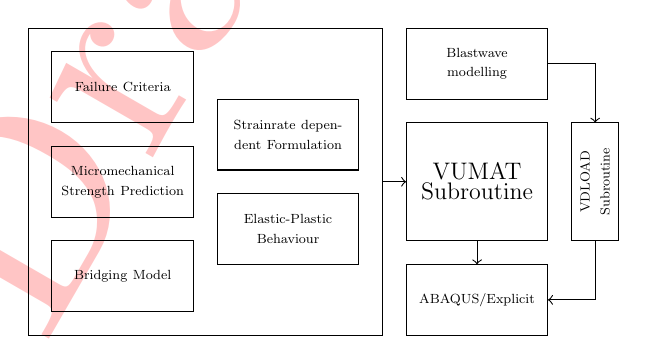
\begin{tikzpicture}[scale=0.6, every node/.style={scale=0.6}]
	\draw (0,0) rectangle (7.5,6.5);
	\draw (0.5,0.5) rectangle (3.5,2) node[pos=.5,text width=3cm,align=center] {\footnotesize Bridging Model};
	\draw (0.5,2.5) rectangle (3.5,4) node[pos=.5,text width=3cm,align=center] {\footnotesize Micromechanical Strength Prediction};
	\draw (0.5,4.5) rectangle (3.5,6) node[pos=.5,text width=3cm,align=center] {\footnotesize Failure Criteria};
	\draw (4,1.5) rectangle (7,3) node[pos=.5,text width=3cm,align=center] {\footnotesize Elastic-Plastic Behaviour};
	\draw (4,3.5) rectangle (7,5) node[pos=.5,text width=3cm,align=center] {\footnotesize Strainrate dependent Formulation};
	
	\draw (8,5) rectangle (11,6.5) node[pos=.5,text width=2.5cm,align=center] {\footnotesize Blastwave modelling};
	
	\draw (8,2) rectangle (11,4.5) node[pos=.5,text width=2.5cm,align=center] {\Large VUMAT Subroutine};
	
	\draw (8,0) rectangle (11,1.5) node[pos=.5,text width=2.5cm,align=center] {\footnotesize ABAQUS/Explicit};
	
	\draw (11.5,2) rectangle (12.5,4.5) node[pos=.5,text width=2.5cm,align=center,rotate=90] {\footnotesize VDLOAD Subroutine};
	
	\draw [->] (7.5,3.25) -- (8,3.25);
	\draw [<-] (9.5,1.5) -- (9.5, 2);
	\draw [<-] (11,0.75) -- (12,0.75) -- (12, 2);
	\draw [->] (11,5.75) -- (12,5.75) -- (12, 4.5);
	
	\end{tikzpicture}
  \caption{Simulation Schematic}
\end{figure}

The material response is studied by integrating the concepts of continuum damage mechanics (CDM), bridging model\cite{ye_zhang_2012} , elasticity and plasticity\cite{zhang_gu_sun_2017}, micromechanics based strength prediction\cite{huang_1999}, strain-rate dependent form-ulation\cite{xin_wen_2015} and a string of failure criteria into the user coded VUMAT subroutine which is used in ABAQUS/Explicit for simulation. In addition to this, the layers of laminates are bonded using surface-based cohesive behavior whereas the interaction between the projectile and the plate is defined using the general contact algorithm. The model consisting of a target plate is having C3D8R elements and the projectile has meshed with R3D4 elements. The mesh is checked for the quality and errors using the metrics such as geometric deviation factor and aspect ratio.

\begin{figure}[h]
  \centering
  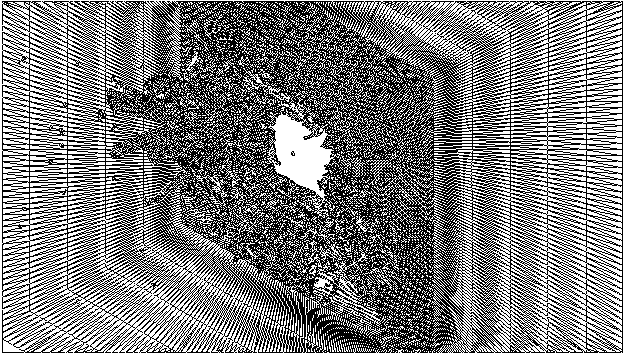
\includegraphics{1.pdf}
  \caption{Back face deformation of 8 layered cross ply laminate under blast loading ($I = 642 MPa$)}
\end{figure}


The blast wave is modeled using the VDLOAD subroutine which contains modified Friedlander equation while considering a near-field blast approach to model time decay and a decoupled approach in modeling spatial decay. The results are obtained using materials Carbon/Epoxy and Glass/Epoxy for simulation. The results of the simulation are validated by the work of performed by previous researchers\cite{bandaru_ahmad_2016}\cite{sevkat_liaw_delale_raju_2009} and was found in good agreement.

\bibliographystyle{unsrt}
\bibliography{bibiliography.bib}

\vspace*{\fill}
\rule{\textwidth}{0.4pt}
\footnotesize \textbf{Full paper access.} This is a shortened version of full research work, and is available on request. Contact at \url{https://mathscapes.xyz/contact}.

\footnotesize \textbf{Usage and permission.} This paper or any portion thereof may not be reproduced or used in any manner whatsoever without the express written permission of Mathscapes Research except for the use of brief quotations in a review.

\end{document}
